%%%%%%%%%%%%%%%%%%%%%%%%%%%%% Define Article %%%%%%%%%%%%%%%%%%%%%%%%%%%%%%%%%%
\documentclass{article}
%%%%%%%%%%%%%%%%%%%%%%%%%%%%%%%%%%%%%%%%%%%%%%%%%%%%%%%%%%%%%%%%%%%%%%%%%%%%%%%

%%%%%%%%%%%%%%%%%%%%%%%%%%%%% Using Packages %%%%%%%%%%%%%%%%%%%%%%%%%%%%%%%%%%
\usepackage{listings, xcolor}
\usepackage{parskip}
\usepackage{hyperref}
\usepackage{amsmath}
\usepackage{graphicx}
\usepackage[a4paper, margin = 1.5cm]{geometry}
\usepackage{float}
\usepackage{amsmath}
\usepackage{amssymb}
\usepackage{parskip}
\usepackage{listings}

\lstset{
frame = shadowbox,
basicstyle = \small\ttfamily,
mathescape = true,
numbers = left,
commentstyle = \itshape\color{gray}
columns = flexible,
keepspaces = true,
moredelim = [l]{//}
}

%%%%%%%%%%%%%%%%%%%%%%%%%%%%%% Title & Author %%%%%%%%%%%%%%%%%%%%%%%%%%%%%%%%
\title{Testing}
\author{Trentin Tommaso}
%%%%%%%%%%%%%%%%%%%%%%%%%%%%%%%%%%%%%%%%%%%%%%%%%%%%%%%%%%%%%%%%%%%%%%%%%%%%%%
\begin{document}
\maketitle
\tableofcontents
\newpage

  \section{Idea}
    Testing = inisieme di attività col fine di dimostrare che un programma svolge i compiti per il quale è stato realizzato, rilevado eventuali difetti prima di renderlo operativo.
    \subsection{Verifica e validazione}
      \begin{itemize}
          \item \textbf{Verifica (Verificaition)}: controllare che SW soddisfi la specifica dei requisiti / gli standard stabiliti all'inizio del ciclo di sviluppo;
          \item \textbf{Validazione (Validation)}: dimostrare che SW risolva il giusto problema, supportando utilizzo atteso e soddisfacendo bisogni degli utenti nell'ambiente operativo.
      \end{itemize}
    \subsection{Testing e debugging}
      Testing rientra nel processo più ampio di Verifica e Validazione (V\&V), è un processo di esecuzione SW allo scopo di scoprire eventuali malfunzionamenti che indicherebbero difetti nel SW.
  \section{Errore / Difetto / Malfunzionamento}
    \subsection{Errore (Error)}
      Situazione frutto di incomprensione da parte di singolo sviluppatore o team di sviluppo, esistono varie tipologie di errori che possono essere commessi:
      \begin{itemize}
          \item Nel tentativo di comprendere requisiti del problema;
          \item Nell'elaborare soluzione al problema;
          \item Nel comprendere / analizzare strumenti;
          \item Nella programmazione (dovuti a distrazione, superficialità...).
      \end{itemize}
    \subsection{Difetto (Fault)}
      Manifestazione nel SW di un errore umano, ha natura \textit{statica} (consiste in codice sintatticamente / semanticamente sbagliato). Se il codice difettoso non viene mai esercitato potrebbe passare inosservato in quanto non causerebbe alcun malfunzionamento durante l'esecuzione.
    \subsection{Malfunzionamento (Failure)}
      Incapacità del SW di comportarsi secondo aspettative / specifiche, ha natura \textit{dinamica} in quanto accade solo in un certo istante e può essere osservato solo mediante esecuzione (più estremo è il crash, altri posssono essere meno evidenti).
    \subsection{Recap}
      \begin{figure}[htpb]
          \centering
          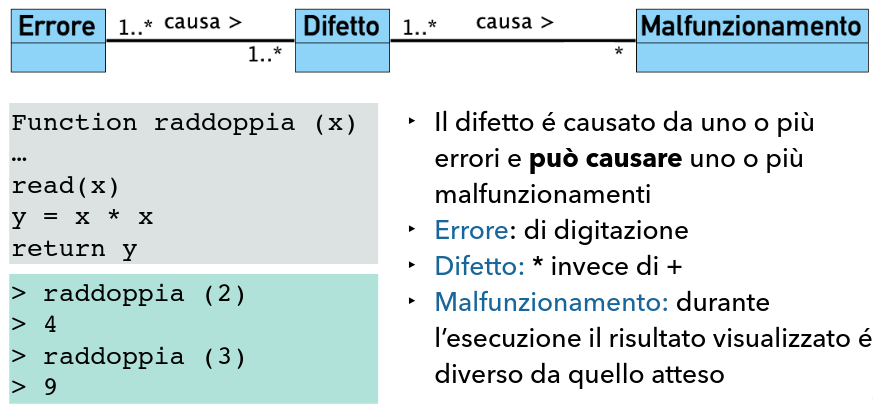
\includegraphics[width=0.7\linewidth]{figures/er_di_ma.png}
      \end{figure}
  \section{Casi di test}
    Durante il testing il SW è esercitato da un insieme di input e ne viene valutato il comportamento, un \textbf{test-case} è particolarmente utile se è in grado di scoprire un malfunzionamento non ancora scoperto da altri. 
    \begin{figure}[htpb]
        \centering
        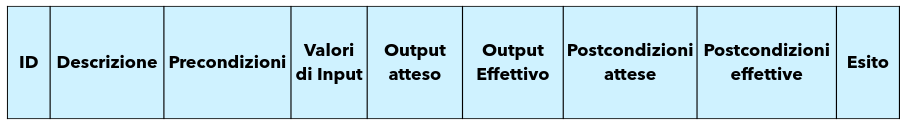
\includegraphics[width=0.8\linewidth]{figures/test_case_par.png}
    \end{figure}
    \begin{itemize}
        \item \textbf{ID} aiuta a specificare / comunicare il caso di test;
        \item \textbf{Descrizione} può indicare requisito che il caso di test intende testare;
        \item \textbf{Precondizioni} sono condizioni da verificare per esecuzione test case;
        \item \textbf{Valori di input} indicano il modo in cui il programma sarà testato;
        \item \textbf{Valori di output attesti} rappresentano comportamento atteso dal SW dopo essere stato esercitato da input specificati;
        \item \textbf{Postcondizioni attese} rappresentano condizioni in cui il sistema dovrebbe trovarsi dopo esecuzione test case;
        \item \textbf{Output effettivo} e \textbf{Postcondizioni effettive} sono valori che vengono conosciuti sono dopo esecuzione del test case;
        \item \textbf{Esito} sarà \textit{malfunzionamento rilevato} se 1+ valori di output / una postcondizione effettivi sono diversi da quelli attesi, \textit{malfunzionamento non rilevato} altrimenti.
    \end{itemize}
    \subsection{Test suite}
      Un caso di test TC$_i$ rileva presenza di 1+ malfunzionamenti se programma P non è corretto per TC$_i$ (produce risultati / postcondizioni diversi dagli attesi). Un insime di test case detto \textbf{test suite} mira a rilevare presenza di più difetti possibili selezionando appropriamente i test case.
    \subsection{Oracolo}
      Conosce comportamento atteso per ogni test case e permette di confrontare risultato atteso con quello effettivo, può essere umano o automatico:
      \begin{itemize}
          \item Generato da specifiche formali;
          \item SW con stesse funzionalità ma sviluppato da altri;
          \item Versione precedente del SW (\textit{test di regressione}).
      \end{itemize}
  \section{Obiettivi}
    \textit{Testing} rivela presenza di malfunzionamenti, non identifica i difetti. \textit{Debugging} è processo di scoperta dei difetti a partire da malfunzionamenti rilevati, si occupa di identificare e rimuovere cause di un malfunzionamento. \textit{Analisi dell'affidabilità} si occupa invece di fornire stima della probabilità che SW operi senza malfunzionamenti per un certo tempo in un certo ambiente.
    \begin{figure}[H]
        \centering
        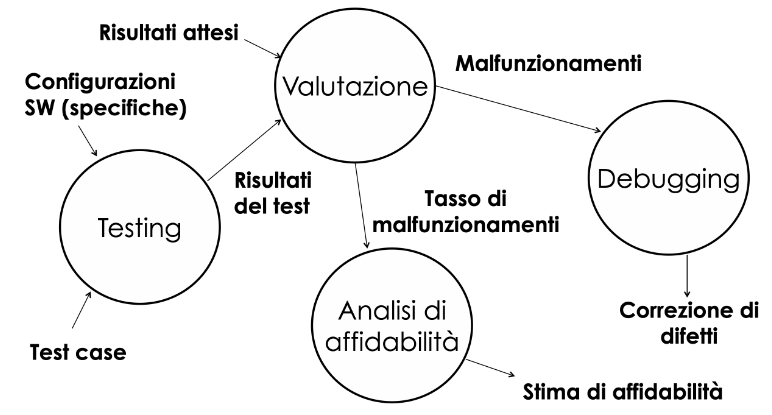
\includegraphics[width=0.5\linewidth]{figures/te_de_af.png}
    \end{figure}
    \subsection{Testing ideale / esaustivo}
      Il testing è \textbf{ideale} se assenza di malfunzionamenti rilevati implica correttezza del programma, è poi \textbf{esaustivo} se contiene tutte le possibili combinazioni dei dati in ingresso al programma (\textit{un test esaustivo è ideale}). In casi non banali il test esaustivo non è pratico e risulta infattibile a causa dei costi elevati, in questi casi selezionano dei casi (\textbf{test selection}) che approssimino al meglio un \textit{test ideale}.
    \subsection{Test selection}
      La bontà di una \textit{test suite} si può misurare in termini di
      \begin{itemize}
          \item \textbf{Efficacia}: \# malfunzionamenti trovati / \# malfunzionamenti da trovare (quasi mai calcolabile in quanto numero da trovare sconosciuto, da privilegiare se si vuole SW affifabile);
          \item \textbf{Efficienza}: \# test che rilevano malfunzionamenti / \# test totali (da privilegiare se si vuole testing meno costoso).
      \end{itemize}
      L'ideale sarebbe trovare maggior numero possibile di malfunzionamenti con minor numero possibile di test case.
    \subsection{Tesi di Dijkstra}
      \textbf{"Test possono dimostrare soltanto la presenza di errori, non la loro assenza"}. Testing pertanto non può dimostrare correttezza SW (in quanto problema indecidibile), deve fornire fiducia nel SW mostrando che è pronto a uso operativo. Un testing che determina assenza di malfunzionamenti può significare al contempo:
      \begin{itemize}
          \item Alta qualità del SW;
          \item Inadeguatezza dei casi di test.
      \end{itemize}
    \subsection{Criteri terminazione / adeguatezza testing}
      Dato che testing esaustivo non fattbile vanno stabiliti criteri per decidere quando testing vada terminato e ritenuto adeguato.
      \begin{itemize}
          \item \textbf{Criterio temporale}: periodo di tempo predefinito;
          \item \textbf{Criterio di costo}: sforzo allocato predefinito;
          \item \textbf{Criterio di copertura}: numero predefinito di obiettivi (linee codice, scenari...) coperti;
          \item \textbf{Criterio statistico}: ultimi k test cases non hanno rilevato malfunzionamenti.
      \end{itemize}
  \section{Testing / Ispezione}
    \begin{itemize}
        \item \textit{Testing} è un'analisi \textbf{dinamica} che mira a rilevare malfunzionamenti di un SW mediante osservazione del suo comportamento e confronto con quello atteso, \textit{è possibile solo per SW che possa essere eseguito}.
        \item \textit{Ispezione} è un'analisi \textbf{statica} che mira a verificare correttezza del SW senza eseguirlo (lettura codice), è possibile anche per SW incompleto o algoritmi non ancora implementati.
    \end{itemize}
    \subsection{Analisi statica}
      \begin{itemize}
          \item \textbf{Vantaggi}
            \begin{itemize}
                \item Malfunzionamenti possono mascherarne altri durante esecuzione dinamica, con analisi statica si possono trovare subito;
                \item Possono venire ispezionate versioni incomplete di un sistema senza costi aggiuntivi;
                \item Ispezione può anche valutare attributi di qualità più generali come conformità a standard e portabilità.
            \end{itemize}
          \item \textbf{Svantaggi}
            \begin{itemize}
                \item Analisi statica può verificare conformità con specifiche ma non quella con necessità utenti;
                \item Analisi statica meno adatta a verificare proprietà funzionali come usabilità.
                \item Difficile rilevare malfunzionamenti dipendenti da valore assunto dinamicamente da variabili.
            \end{itemize}
      \end{itemize}
  \section{Livelli del testing}
    \begin{itemize}
        \item \textbf{Test dei componenti (d'unità)}: test di singole unità del SW;
        \item \textbf{Test d'integrazione}: integra diversi componenti tra loro per rilevare problemi d'interazione;
        \item \textbf{Test di sistema}: SW testato dopo integrazione di tutti i componenti;
        \item \textbf{Test di accettazione}: condotti da utente finale per validare i requisiti.
    \end{itemize}
    \subsection{Test d'unità}
      Ciascuna unità viene verificata, spesso in fase di implementazione, in base alla propria documentazione. Le unità da testare possono essere:
      \begin{itemize}
          \item Metodi di una classe;
          \item Classi;
          \item Componenti riusabili che offrono specifica interfaccia per accedere alle loro funzionalità.
      \end{itemize}
      \subsubsection{Test d'unità automatizzato}
        Test delle unità può essere oneroso, quinsi hanno successo strategie di automatizzazione, la più banale è il \textbf{main-based approach} che fornisce a ogni unità un test method con codice per esercitare le funzionalità. Causa però \textbf{problemi}:
        \begin{itemize}
            \item main aggiuntivo sarà distribuito nel prodotto finale;
            \item per testare componenti alternativi saranno necessari più metodi nel main.
        \end{itemize}
        \begin{figure}[htpb]
            \centering
            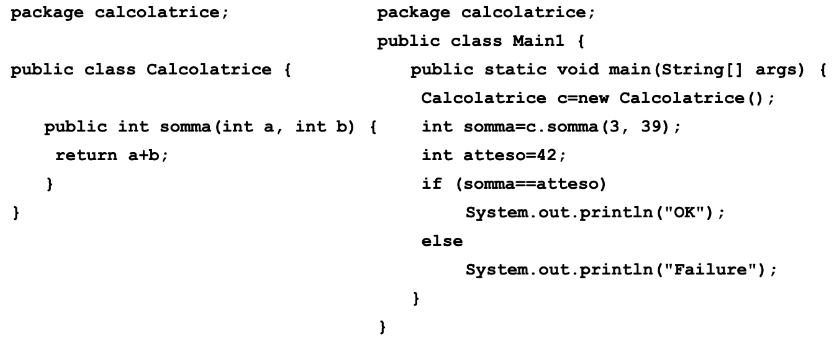
\includegraphics[width=0.7\linewidth]{figures/main_based_es.png}
        \end{figure}
    \subsection{Test d'integrazione}
      Richiede costruzione incrementale del sistema partendo da componenti testati singolarmente (aggiungendo una funzionalità alla volta): anche se quest'ultimi sono ritenuti corretti va verificata eventuale presenza di malfunzionamenti tra i moduli (possibili problemi delle interfacce). 
      \subsubsection{Test di regressione}
        Possibile che dopo una modifica SW sia "regredito" (modifica abbia introdotto difetti prima non presenti), dopo ciascuna integrazione vanno quindi rieffettuati i test precedenti per effettuare non ci siano nuovi malfunzionamenti del vecchio codice.
      \subsubsection{Stub / Driver}
        Moduli guida (\textbf{driver}) simulano i componenti chiamati, accettando dati del test case, invocando componente chiamato e stampando i risultati. I moduli fittizzi (\textbf{stub}) invece simulano i componenti gerarchicamente inferiori al componente da testare: sono invocati dal componente testato, simulano funzionamento del componente chiamato mediante funzioni fittizie (correttezza vera per ipotesi). Driver e stub sono un overhead in quando devono essere implementati pur non facendo parte del prodotto finale.
        \begin{figure}[htpb]
            \centering
            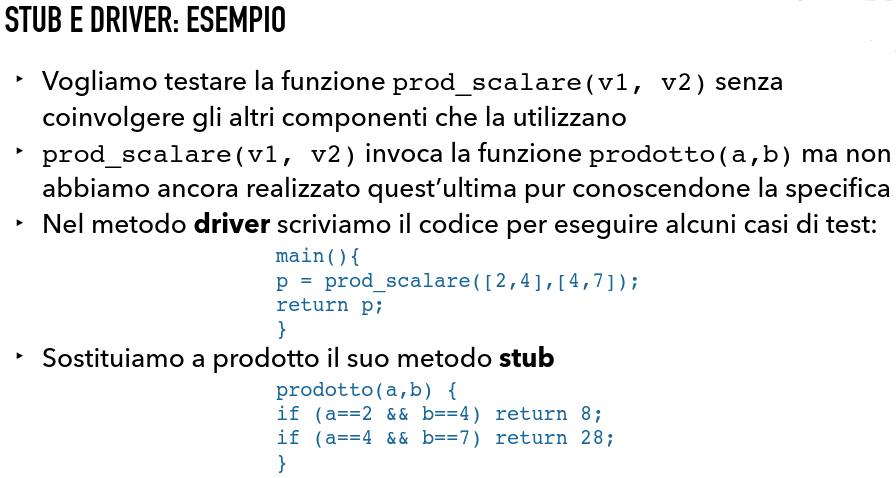
\includegraphics[width=0.7\linewidth]{figures/dr_st_es.png}
        \end{figure}
    \subsection{Test di sistema}
      SW è testato dopo essere stato integrato (anche con altri elementi di sistema come HW e dati). Ha come scopo la verifica che tutti gli elementi del sistema siano correttamente integrati e che il sistema complessivo soddisfi i requisiti.
    \subsection{Test di accettazione}
      Test condotti dall'utente finale per consentire validazione di tutti i requisiti:
      \begin{itemize}
          \item \textbf{$\alpha$-Test} condotto da team selezionato di clienti e/o utilizzatori finali che avviene in ambiente controllato presso lo sviluppatore;
          \item \textbf{$\beta$-Test} condotto da numero maggiore di utenti finali con proprio HW che possono avere interazioni non previste con SW, sviluppatore solitamente non presente; oltre a essere una forma di commercializzazione può rivelare nuovi difetti / incompatibilità.
      \end{itemize}
\end{document}

